\chapter{Conifer Broadleaf Forest: Patterns, Processes and Hypotheses}%
\label{ch:coniferpatterns}

This chapter will be largely based on the common type of conifer broadleaf forest found throughout the country on adequately drained and reasonably fertile soils.
It comprises a mixture of conifers mostly of the family Podocarpaceae; herbaceous and woody flowering plants; and ferns.

The features of other more restricted types will be considered later: well drained coastal forest without conifers; \IDX{kauri} (\BotanicRef{Agathis australis}[Agathis][australis]) dominated forest in the warmer northern North Island on less fertile, but well drained soils; \IDX{manawa} (\BotanicRef{Avicennia resinifera}[Avicennia][resinifera], \IDX{mangrove}) low forest at similar latitudes in the intertidal zone; and freshwater swamp and bog forests.

\section{Distribution}

At the time of European settlement early last century, conifer broadleaf forest was the most widespread type of vegetation in the North Island\figureref{\fullref{fig:1vegetationpatterns}} and also occupied several disjunct areas through the South Island and in Fiordland.
It is believed that before people first set foot in New Zealand about 1100 years ago, conifer broadleaf forest was even more extensive, largely occupying pre-European fire-induced fern and shrubland regions in the North Island and the grasslands and shrublands in the east and south of the South Island.
The evidence for this will be reviewed in Chapter~\ref{ch:openhabitats} \nameref{ch:openhabitats}.

Over the wide latitudinal range of the New Zealand conifer broadleaf forest, from \SIrange{34}{47}{\degree}S (\ang{50}S if the \IDX{southern rata}[rata!southern] (\BotanicRef{Metrosideros umbellata}[Metrosideros][umbellata]) forest of the Auckland Islands is included), the total number of species decreases as one goes from north to south, with a tendency towards an aggregation of southern limits at the middle latitude of the North Island, \ang{38}S, and at \ang{42}S in the northern South Island.

\section{The Commoner Species of the Forest Strata}

\subsection{Emergents}

Conifers are prominent in this usually discontinuous stratum, with \IDX{rimu} (\BotanicRef{Dacrydium cupressinum}[Dacrydium][cupressinum]) the most common in a range of reasonably moist sites on flats, slopes and ridges.
The light-demanding and drought tolerant \IDX{totara} (\BotanicRef{Podocarpus totara}[Podocarpus][totara]) favours stony river terraces and similar level areas, while \IDX{kahikatea} (\BotanicRef{Dacrycarpus dacrydioides}[Dacrycarpus][dacrydioides]) prefers moister places often near streams.
\IDX{Miro}[miro] (\BotanicRef{Prumnopitys ferruginea}[Prumnopitys][ferruginea]), the most shade tolerant of the conifers, and \IDX{matai} (\BotanicRef{Prumnopitys taxifolia}[Prumnopitys][taxifolia]) are not quite so tall as the three preceding species and are not always emergent.
Miro occupies a similar range of sites to \IDX{rimu}, and \IDX{matai} is most abundant on fertile alluvial or volcanic ash soils.
As \IDX{totara}, \IDX{kahikatea} and \IDX{matai} thrive on younger fertile soils they are most prominent during the first centuries of forest development.

Although not tall trees, at higher altitudes \IDX{Hall's totara}[totara!Hall's] (\BotanicRef{Podocarpus hallii}[Podocarpus][hallii]) and the attractive conical mountain cedar or \IDX{kaikawaka} (\BotanicRef{Libocedrus bidwillii}[Libocedrus][bidwillii]) may be emergent above a low forest canopy.

Some flowering trees also contribute to this stratum: \IDX{northern rata}[rata!northern] (\BotanicRef{Metrosideros robusta}[Metrosideros][robusta]) because it commences its life on a \IDX{rimu} or other tall tree; \IDX{pukatea} (\BotanicRef{Laurelia novae-zelandiae}[Laurelia][novae-zelandiae]) in association with \IDX{kahikatea} in moist places; and \IDX{rewarewa} (\BotanicRef{Knightia excelsa}[Knightia][excelsa]).
The last with its distinctive `lombardy poplar' form is sometimes abundant on hill slopes, but usually in relatively young forests.

The emergent conifers range throughout the country.
Of the three flowering trees \IDX{rewarewa} and \IDX{northern rata}[rata!northern] reach their southern limits in the northern South Island, while \IDX{pukatea} extends to Fiordland on the west.

\subsection{Canopy}

North of \ang{36}S on the Northland Peninsula, \IDX{taraire} (\BotanicRef{Beilschmiedia tarairi}[Beilschmiedia][tarairi]), with its broad mesophyll leaves, dominates the canopy, usually in association with \IDX{kamahi}'s northern relative \IDX{towai} (\BotanicRef{Weinmannia silvicola}[Weinmannia][silvicola]).
At higher altitudes in Northland, \IDX{taraire}'s relative \IDX{tawa} (\BotanicRef{Beilschmiedia tawa}[Beilschmiedia][tawa]), with its smaller, willow-like leaves, is a minor component of the canopy, but from about \ang{36}S it replaces \IDX{taraire} as the dominant at low altitudes and continues in this role as far as the north-east of the South Island at \ang{42}S.
Succeeding \IDX{tawa} altitudinally as the canopy dominant in the North Island from about \ang{39}S is \IDX{kamahi} (\BotanicRef{Weinmannia racemosa}[Weinmannia][racemosa]); it also replaces \IDX{tawa} in the lowland conifer broadleaf forests of most of the South Island and Fiordland.

Several other species also contribute to the canopy.
\IDX{Puriri}[puriri] (\BotanicRef{Vitex lucens}[Vitex][lucens]), which has strong tropical affinities, is limited to the northern half of the North Island; \IDX{tanekaha} or \IDX{celery pine} (\BotanicRef{Phyllocladus trichomanoides}[Phyllocladus][trichomanoides]) and \IDX{black maire} (\BotanicRef{Nestegis cunninghamii}[Nestegis][cunninghamii]) reach the northern South Island.\footnote{Tanekaha is absent from the southern North Island.}
\IDX{Hinau}[hinau] (\BotanicRef{Elaeocarpus dentatus}[Elaeocarpus][dentatus]) reaches the central South Island, while its higher altitude relative \IDX{pokaka} (\BotanicRef{Elaeocarpus hookerianus}[Elaeocarpus][hookerianus]) reaches Fiordland.

On the west and south of the South Island \IDX{southern rata}[rata!southern] (\BotanicRef{Metrosideros umbellata}[Metrosideros][umbellata]) contributes to the canopy of \IDX{kamahi} forests.

\subsection{Subcanopy Trees}

Two species of decidedly tropical aspect reach the northern South Island, although they are never far from the sea in the southern parts of their ranges.
These are \IDX{kohekohe} (\BotanicRef{Dysoxylum spectabile}[Dysoxylum][spectabile]) with its large, pinnately compound leaves and our sole native species of palm, the \IDX{nikau}[nikau palm] (\BotanicRef{Rhopalostylis sapida}[Rhopalostylis][sapida])\footnote{The nikau palm reaches its southern limit on the Chatham Islands at \ang{44}S.}\figureref{\fullref{fig:60nikau}}.

\begin{SCfigure}[2.0][!t]
	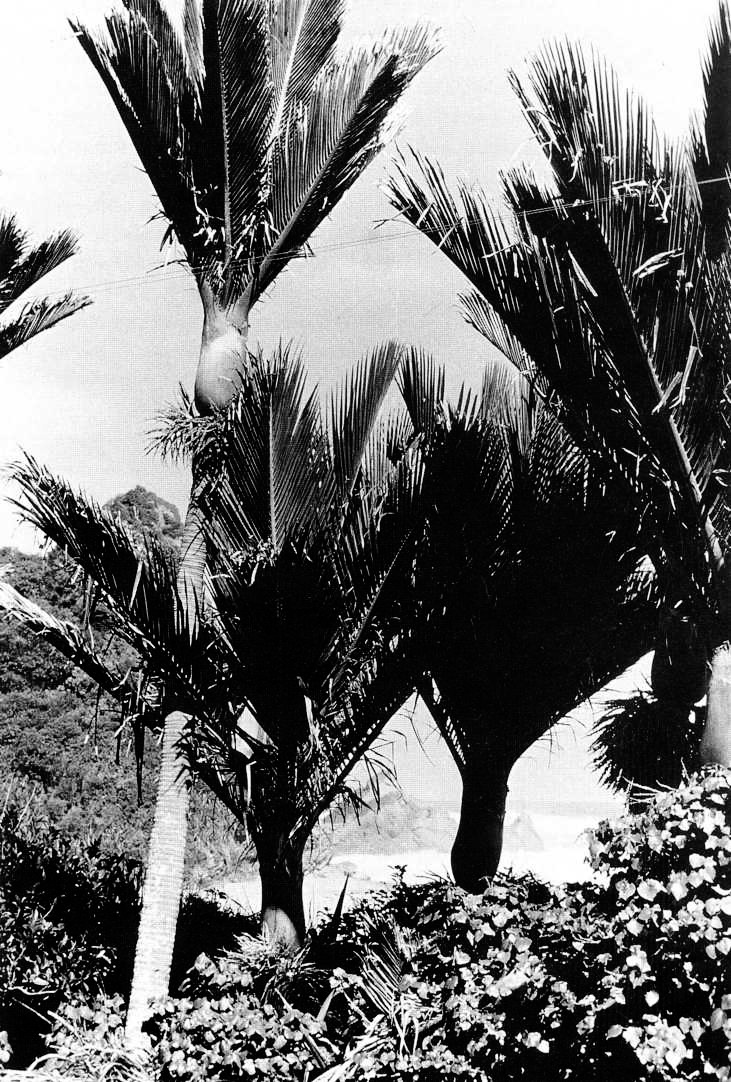
\includegraphics[width=0.66\textwidth]{graphics/figure60nikau.jpg}
	\centering
	\caption[A grove of nikau palms]{A grove of \IDX{nikau palm}s (\BotanicRef{Rhopalostylis sapida}[Rhopalostylis][sapida]) growing near the sea at \ang{42}S on the west coast of the South Island south of Westport. Photo:  J. W. Dawson.}%
	\label{fig:60nikau}
\end{SCfigure}

Other species which tend to be more wide ranging are \IDX{mahoe} (\BotanicRef{Melicytus ramiflorus}[Melicytus][ramiflorus]), \IDX{porokaiwhiri} (\BotanicRef{Hedycarya arborea}[Hedycarya][arborea], \IDX{pigeonwood}), \IDX{toro} (\BotanicRef{Myrsine salicina}[Myrsine][salicina]) and two common tree ferns: \IDX{mamaku} or \IDX{black tree fern} (\BotanicRef{Cyathea medullaris}[Cyathea][medullaris]) and \IDX{ponga} or \IDX{silver tree fern} (\BotanicRef{Cyathea dealbata}[Cyathea][dealbata]).
Some of these species are most abundant in canopy gaps, while other small trees, are largely restricted to such sites within the forest; for example, \IDX{makomako} (\BotanicRef{Aristotelia serrata}[Aristotelia][serrata], \IDX{wineberry}), \IDX{putaputaweta} (\BotanicRef{Carpodetus serratus}[Carpodetus][serratus]), \IDX{kaikomako} (\BotanicRef{Pennantia corymbosa}[Pennantia][corymbosa]), \IDX{kotukutuku} (\BotanicRef{Fuchsia excorticata}[Fuchsia][excorticata]), \IDX{houhere} (\BotanicRef{Hoheria populnea}[Hoheria][populnea], \IDX{lacebark}), several species of \BotanicRef{Pittosporum}, \IDX{horoeka} (\BotanicRef{Pseudopanax crassifolius}[Pseudopanax][crassifolius], \IDX{lancewood}) and the \IDX{ti kouka} (\BotanicRef{Cordyline australis}[Cordyline][australis], \IDX{cabbage tree}).

A few other small trees prefer higher altitudes in northern New Zealand and they include \IDX{kapuka} (\BotanicRef{Griselinia littoralis}[Griselinia][littoralis], \IDX{broadleaf}) and the \IDX{mountain cabbage tree}[cabbage tree!mountain] (\BotanicRef{Cordyline indivisa}[Cordyline][indivisa], \IDX{toi}).
The latter with its unbranched trunk and massive head of broad, silvery-green leaves is certainly the most handsome of our cordylines\figureref{\fullref{fig:61cabbagetree}}.
It looks as if it would be at home on a tropical strand, so it seems strange that it should favour moister, cooler, montane forests.

\begin{SCfigure}[2.0][t]
	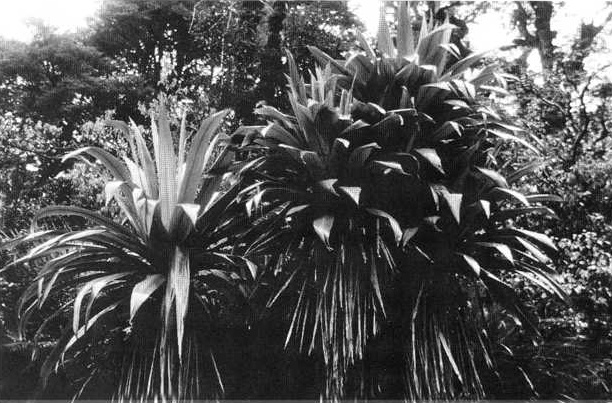
\includegraphics[width=0.66\textwidth]{graphics/figure61cabbagetree.jpg}
	\centering
	\caption[The mountain cabbage tree]{The \IDX{mountain cabbage tree}[cabbage tree!mountain] (\BotanicRef{Cordyline indivisa}[Cordyline][indivisa]).
	Photo: J. W. Dawson.}%
	\label{fig:61cabbagetree}
\end{SCfigure}

\subsection{Shrubs}

\IDX{Kawakawa}[kawakawa] (\BotanicRef{Macropiper excelsum}[Macropiper][excelsum]) is a distinctive undershrub with heart shaped leaves and jointed stems.
\IDX{Kawakawa}[kawakawa] is sometimes called `native pepper tree' because of its hot tasting leaves, and it is in fact related to the true pepper plant of Indonesia.
It is also related to the similarly named kava plant of Fiji.
\IDX{Horopito}[horopito] (\BotanicRef{Pseudowintera axillaris}[Pseudowintera][axillaris]) with its dark green shiny leaves has also been termed `pepper tree' for the same reason, but it is not in fact related to \IDX{kawakawa}.
It belongs to the Winteraceae, a family often considered to be the most primitive of the flowering plants.

Other common shrubs are the thin-leaved \IDX{hangehange} (\BotanicRef{Geniostoma rupestre}[Geniostoma][rupestre]), \IDX{kanono} (\BotanicRef{Coprosma grandifolia}[Coprosma][grandifolia]) and \IDX{pate} (\BotanicRef{Schefflera digitata}[Schefflera][digitata]) with its large palmately compound leaves.
The tree fern, \IDX{wheki} (\BotanicRef{Dicksonia squarrosa}[Dicksonia][squarrosa]), may also be common.
It is notable for spreading by horizontal stems or rhizomes to form groves.

In better lit places \IDX{whauwhaupaku} (\BotanicRef{Pseudopanax arboreus}[Pseudopanax][arboreus], \IDX{five-finger}) may occur.
Its leaves are of similar form to those of \IDX{pate} but they have a thicker texture and are more coarsely toothed at the margins.
Accompanying species may be the two common larger-leaved coprosmas both known as \IDX{karamu}: \BotanicRef{Coprosma robusta}[Coprosma][robusta] and \BotanicRef{Coprosma lucida}[Coprosma][lucida], the bubbly-leaved \IDX{ramarama} (\BotanicRef{Lophomyrtus bullata}[Lophomyrtus][bullata]), \IDX{wharangi} (\BotanicRef{Melicope ternata}[Melicope][ternata]), the `tree daisies' \IDX{heketara} (\BotanicRef{Olearia rani}[Olearia][rani]) and the familiar large-leaved \IDX{rangiora} (\BotanicRef{Brachyglottis repanda}[Brachyglottis][repanda]).

Among the undershrubs which occur at higher altitudes in the north are \IDX{mountain horopito} (\BotanicRef{Pseudowintera colorata}[Pseudowintera][colorata]), often with an extremely attractive red or yellow leaf colouration; \IDX{mountain five-finger} (\BotanicRef{Pseudopanax colensoi}[Pseudopanax][colensoi]), \IDX{haumakoroa} (\BotanicRef{Pseudopanax simplex}[Pseudopanax][simplex]), the tree fern \IDX{katote} (\BotanicRef{Cyathea smithii}[Cyathea][smithii]) and \IDX{stinkwood} (\BotanicRef{Coprosma foetidissima}[Coprosma][foetidissima]).

The coprosma is sometimes known as `stinkwood' because the crushed leaves smell like rotten cabbage.
Indeed the name of the genus is based on this species, `copros' being latin for dung.
Insult is added to injury with the species name, so that \BotanicRef{Coprosma foetidissima}[Coprosma][foetidissima] could be translated as `stinking dung plant'.
In fact very few of the many species of \BotanicRef{Coprosma} have an unpleasant smell.

\BotanicRef{Alseuosmia pusilla}[Alseuosmia][pusilla] is a small shrub which is often overlooked since it frequently grows with \IDX{mountain horopito} and looks very much like it.
In the absence of flowers or berries the easiest way to tell them apart is to turn over the leaves --- those of \IDX{horopito} are white, those of \BotanicRef{Alseuosmia} pale green.
It has been suggested that, as the peppery leaves of \IDX{horopito} are unpalatable to deer they may also have been unpalatable to moas.\footnote{\cite{greenwood1977evolution}}
In that case moas, like many bush lovers today, may have passed \BotanicRef{Alseuosmia pusilla}[Alseuosmia][pusilla] by.
The genus \BotanicRef{Alseuosmia} seems to specialise in such mimicry.
I have seen a form of this genus in a forest near Kaitaia with round bullate (bubbly) leaves, and I took it at first to be the familiar \IDX{ramarama} (\BotanicRef{Lophomyrtus bullata}[Lophomyrtus][bullata]).

\subsection{Ground Plants}

The most abundant plants on the forest floor are ferns, but flowering plants may also be found.
Many of the ferns belong to such widespread genera as \BotanicRef{Asplenium}, \BotanicRef{Blechnum}, \BotanicRef{Polystichum} and the membranous leaved filmy ferns (\BotanicRef{Hymenophyllum} and \BotanicRef{Trichomanes}).
The two species of \BotanicRef{Leptopteris}, although larger than the filmy ferns and not related to them, have similar membranous leaves.
The famous \IDX{heruheru} (\BotanicRef{Leptopteris superba}[Leptopteris][superba], \IDX{crepe fern}) favours moist, shady, cool situations and owes its attractively fluffy leaf texture to the ultimate leaf segments, which are set at right angles to the plane of the leaf\figureref{\fullref{fig:62crepefern}}.

Among flowering plants, species of \BotanicRef{Astelia} form large tussocks; the \IDX{bush rice grass} (\BotanicRef{Microlaena avenacea}[Microlaena][avenacea]) covers the ground in places and in season the flowers of species of such orchid genera as \BotanicRef{Corybas} and \BotanicRef{Pterostylis} make their appearance.
In the north, moist shady banks may be completely covered by attractive mosaics of the reddish-purple tinted leaves of \IDX{parataniwha} (\BotanicRef{Elatostema rugosum}[Elatostema][rugosum])\figureref{\fullref{fig:63parataniwha}}.

\begin{figure}[!b]
	% Outer minipage scaled to limit width.
	% Inner minipages scaled so the images have the same height.
	\begin{minipage}[t]{\textwidth}
		\begin{minipage}[t]{(\textwidth-\fgap) * \real{0.497}}
			\centering
			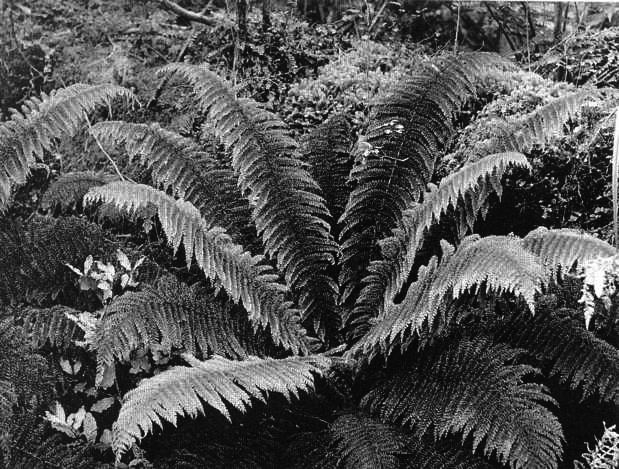
\includegraphics[width=\textwidth]{graphics/figure62crepefern.jpg}
			\caption[Heruheru (\emph{Leptopteris superba}, crepe fern)]{Heruheru (\BotanicRef{Leptopteris superba}[Leptopteris][superba], crepe fern).
			Photo: National Publicity Studios.}%
			\label{fig:62crepefern}
		\end{minipage}\hspace{\fgap}%
		\begin{minipage}[t]{(\textwidth-\fgap) * \real{0.503}}
			\centering
			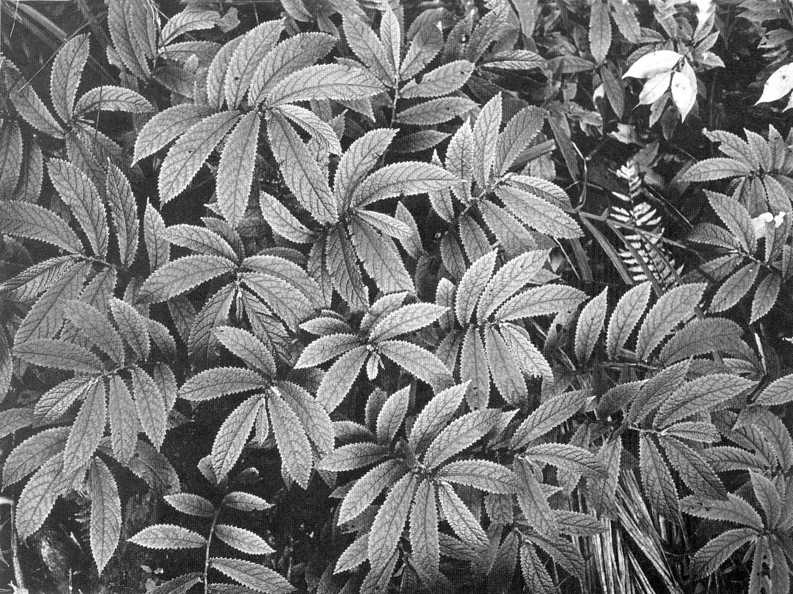
\includegraphics[width=\textwidth]{graphics/figure63parataniwha.jpg}
			\caption[Parataniwha]{Parataniwha (\BotanicRef{Elatostema rugosum}[Elatostema][rugosum]).
			In forest south of Kaitaia, far northern North Island.
			Photo: J. W. Dawson.}%
			\label{fig:63parataniwha}
		\end{minipage}
	\end{minipage}
\end{figure}

\section{Life History of the New Zealand Conifer Broadleaf Forest}

There are a number of theories on this topic.

\subsection[Linear Succession (Climax)]{Linear Succession (Climax)}


A postulated sequence\footnote{\cite{cockayne1928vegetation}}\footnote{\cite{mckelvey1963synecology}}\footnote{\cite{mckelvey1973pattern}}\figureref{\fullref{fig:64forestsuccession}} which leads to the present forests, with their overstorey of scattered podocarps and canopy of flowering trees, is as follows:

\begin{figure}[!b]
	\centering
	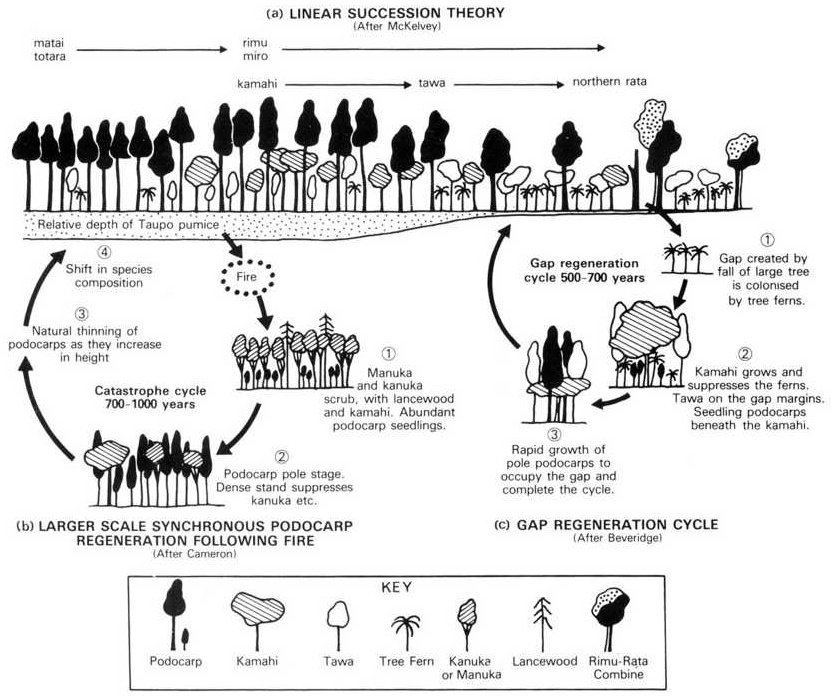
\includegraphics[width=\textwidth]{graphics/figure64forestsuccession.jpg}
	\caption[Linear and cyclic forest successions]{Linear and cyclic forest successions. (Reproduced with permission from \emph{To Save a Forest---Whirinaki.})}%
	\label{fig:64forestsuccession}
\end{figure}

Where the previous forest cover is completely removed by such agents as volcanism or fire, the first coloniser is \IDX{rarauhe} (\BotanicRef{Pteridium esculentum}[Pteridium][esculentum], \IDX{bracken fern}) followed in order by two small-leaved light demanding species --- the shrub \IDX{manuka} (\BotanicRef{Leptospermum scoparium}[Leptospermum][scoparium]) and the small tree \IDX{kanuka} (\BotanicRef{Kunzea ericoides}[Kunzea][ericoides])

Within this association, broader-leaved shrubs and small trees establish, including \IDX{whauwhaupaku} (\BotanicRef{Pseudopanax arboreus}[Pseudopanax][arboreus], \IDX{five-finger}), \IDX{horoeka} (\BotanicRef{Pseudopanax crassifolius}[Pseudopanax][crassifolius], \IDX{lancewood}), \IDX{karamu} (\BotanicRef{Coprosma lucida}[Coprosma][lucida]), \IDX{kohukohu} (\BotanicRef{Pittosporum tenuifolium}[Pittosporum][tenuifolium]), juvenile \IDX{rewarewa} (\BotanicRef{Knightia excelsa}[Knightia][excelsa]), juvenile \IDX{kamahi} (\BotanicRef{Weinmannia racemosa}[Weinmannia][racemosa]), and in moister places the tree ferns \IDX{mamaku} (\BotanicRef{Cyathea medullaris}[Cyathea][medullaris]) and \IDX{ponga} (\BotanicRef{Cyathea dealbata}[Cyathea][dealbata]), \IDX{mahoe} (\BotanicRef{Melicytus ramiflorus}[Melicytus][ramiflorus]), \IDX{makomako} (\BotanicRef{Aristotelia serrata}[Aristotelia][serrata], \IDX{wineberry}), \IDX{kotukutuku} (\BotanicRef{Fuchsia excorticata}[Fuchsia][excorticata], \IDX{tree fuchsia}) and \IDX{pate} (\BotanicRef{Schefflera digitata}[Schefflera][digitata]).

When these broad-leaved plants form a canopy the bracken, \IDX{manuka} and \IDX{kanuka} gradually die out as the light falls below the level required for their continued recruitment.
It is at this stage, about 50 years from the beginning of the sequence, when the forest floor is sheltered but still quite well-lit, that the podocarp conifers become established.
After a further 50 years or so the podocarps begin to grow above the broadleaf canopy and by the time they form a higher stratum themselves, the lower layer of flowering trees is now dominated by \IDX{kamahi} (\BotanicRef{Weinmannia racemosa}[Weinmannia][racemosa]), often initially epiphytic on the \IDX{ponga} tree fern, with scattered \IDX{rewarewa}s (\BotanicRef{Knightia excelsa}[Knightia][excelsa]), \IDX{hinau} (\BotanicRef{Elaeocarpus dentatus}[Elaeocarpus][dentatus]) and maire (\BotanicRef{Nestegis cunninghamii}[Nestegis][cunninghamii]\index{black maire} and \BotanicRef{Nestegis lanceolata}[Nestegis][lanceolata]\index{white maire}).

Finally, shade-demanding species enter and \IDX{tawa} (\BotanicRef{Beilschmiedia tawa}[Beilschmiedia][tawa]) largely replaces \IDX{kamahi} in the forest canopy.
The forest floor is now strongly shaded and the podocarps, light-demanding to varying degrees, no longer establish.
The podocarp trees which are already present, often in combination with epiphytic \IDX{northern ratas}[rata!northern] (\BotanicRef{Metrosideros robusta}[Metrosideros][robusta]), gradually die out and the climax, according to this hypothesis, is a forest with the canopy dominated by \IDX{tawa} and without emergents.
The \IDX{tawa} and other shade-demanding species are able to maintain themselves indefinitely until some catastrophic event destroys the forest to initiate a new succession.

\subsection[Cycles]{Cycles}

Field\figureref{\fullref{fig:64forestsuccession}} observations by a number of botanists have led to some questioning of the above sequence of events.
Some have suggested that, rather than there being a succession leading to a climax, there may in fact be repetitive cycles.
For example, on the volcanic plateau of the central North Island it has been observed in forests with emergent podocarps over a main canopy of \IDX{kamahi}, or \IDX{kamahi} and \IDX{tawa}, that where a podocarp falls the gap is occupied by tree ferns.
\IDX{Kamahi}[kamahi] establishes epiphytically on the tree ferns and podocarps then regenerate under the \IDX{kamahi} and eventually overtop them.\footnote{\cite{cameron1955mosaic}}\footnote{\cite{beveridge1973regeneration}} A similar sequence has been observed in south Westland.\footnote{\cite{poole1937survey}}

Probably because of their importance as timber trees, the lack of regeneration of podocarps in some New Zealand conifer broadleaf forests has received particular attention.
According to the successional and cyclic hypotheses just reviewed this would be a normal consequence of forest development.

\subsection{Climate Change}

Holloway\footnote{\cite{holloway1954forests}} suggested that the general lack of regeneration of podocarps since the time when the present mature to aging emergents established is due to a climate change to colder and drier conditions from about 1300 A.D.
Holloway based his climate change hypothesis on forest patterns in western Southland, in which he saw evidence of a downward movement of vegetational zones, and on historical and other evidence of a worldwide colder interval, the `Little Ice Age', during the last millenium.

Wardle\footnote{\cite{wardle1963regeneration}} investigated a number of podocarp-dominated stands on the west and east of the South Island and in Fiordland.
He supported Holloway's hypothesis but concluded that the `regeneration gap' started later than Holloway suggested, from about 1600 to 1800 A.D., and that it was most marked in the drier eastern South Island and least marked on the wetter west and in Fiordland.
Since about 1800 the regeneration of podocarps has resumed at some localities.

\subsection{Angiosperm Forest Dominance}

According to a more dramatic interpretation of the dynamics of the New Zealand conifer broadleaf forest put forward by Robbins,\footnote{\cite{robbins1962podocarp}} it is not in fact one forest, but two in competition --- one comprising the conifers and the other the flowering trees.
The conifers belong to a more ancient and less specialised group of plants, which along with ferns and their allies formed forests in New Zealand before flowering plants became dominant throughout the world.
Following the establishment of the more specialised flowering trees in New Zealand the less specialised conifers, he suggests, have been on the road to extinction.
Their present poor regeneration is seen as a reflection of this trend.
Only where raw new soil conditions, unsuitable for most flowering trees, are brought about by volcanism or glaciation can the conifers still form dense forests and even these give way to flowering trees as more mature soils develop.

The validity of this interpretation can be questioned.
Firstly, conifers have coexisted with angiosperms in New Zealand for 100 million years, so it seems unlikely that they will disappear for some time to come.
Secondly, if the conifers are doomed to extinction because they are more ancient and less specialised, wouldn't this be even more true for the ferns, an older and less specialised group than the conifers? In fact ferns are abundant in New Zealand forests and give no cause for any belief that they are on the road to extinction.
The probable truth of the matter is that when a more specialised plant or animal group becomes dominant throughout the world, many members of the preceding dominant group become extinct; but there is no reason why the survivors could not evolve new forms suited to the changed conditions.
This would certainly appear to be true for the ferns as most forest ferns belong to an advanced group, which came into existence at about the same time as the now dominant angiosperms and diversified with them.
The tree ferns and filmy ferns are more ancient groups but they give every indication of being permanent components of the conifer broadleaf forests.

As far as conifers are concerned New Zealand is not the only place where apparently inadequate regeneration in mature forests has been noted.
It has been observed in forests of Melanesia with species of \BotanicRef{Araucaria}\footnote{\cite{havel1971araucaria}} and \BotanicRef{Agathis},\footnote{\cite{whitmore1966social}} and similar extinction hypotheses have been proposed.
Studies in both areas have been carried out to test the validity of these hypotheses and they have all concluded that the conifers concerned have a permanent role in the forests as a result of recurring natural disturbances.
In New Zealand a similar investigation\footnote{\cite{veblen1982conifer}} has been made into the role of \IDX{pahautea} (\BotanicRef{Libocedrus bidwillii}[Libocedrus][bidwillii], \IDX{NZ cedar}) in a number of montane rain forests in the South Island and the same conclusion has been drawn.

This seems to suggest then that the failure of emergent conifers (as indeed of many tropical angiosperm emergents\footnote{\cite{whitmore1975tropical}}\footnote{\cite{jones1956ecological}}) to regenerate under a dense canopy is a normal feature of rain forest development, and that special climatic and evolutionary hypotheses are unnecessary.

\section{More Restricted Forest Types}

\subsection{Coastal Forest}

This type is not greatly different from the general conifer broadleaf forest of better drained sites.
It is best developed along the Northland coasts and adjacent islands and is dominated by three species that rarely occur very far from the sea.
\IDX{Pohutukawa}[pohutukawa] (\BotanicRef{Metrosideros excelsa}[Metrosideros][excelsa]), which often grows alone on coastal cliffs, is restricted to the northern half of the North Island, but \IDX{karaka} (\BotanicRef{Corynocarpus laevigatus}[Corynocarpus][laevigatus]) with its large, dark green leathery leaves and \IDX{ngaio} (\BotanicRef{Myoporum laetum}[Myoporum][laetum]) extend to the northern and eastern South Island.

Coastal forest is of lower stature than inland forest and, as a result of the general absence of conifers, it lacks emergents.

In addition to the three trees already mentioned, of which \IDX{pohutukawa} is the largest (and when in flower the most spectacular with its bright red stamens) there may be a number of other trees, shrubs and herbs.
Many of these also occur in inland forests, at least in the far north.
Notable among these are the trees \IDX{puriri} (\BotanicRef{Vitex lucens}[Vitex][lucens]), \IDX{kohekohe} (\BotanicRef{Dysoxylum spectabile}[Dysoxylum][spectabile]) and the shrub \IDX{kawakawa} (\BotanicRef{Macropiper excelsum}[Macropiper][excelsum]).

Of particular note are a number of large-to very large-leaved species in the northern North Island which range from moderately common to rare.
Some of them have strong tropical affinities, and so can be regarded as relics from warmer times.

On the mainland as well as on islands, and extending to East Cape and beyond, are the small trees \IDX{parapara} or the `bird catching tree' (\BotanicRef{Pisonia brunoniana}[Pisonia][brunoniana]) and \IDX{tawapou} (\BotanicRef{Planchonella costata}[Planchonella][costata]).
\IDX{Parapara}[parapara] has extremely sticky fruits to which small birds can become attached.
It is also found in Australia and some Pacific Islands.
The \IDX{tawapou} is closely related to species in Norfolk Island and Fiji.

The remaining species are found on the Three Kings Islands\footnote{\cite{baylis1948vegetation}}\footnote{\cite{oliver1948flora}} off the northern tip of New Zealand and are either restricted there to or also occur on the Hen and Chicken Islands or Poor Knights Islands further south.

\begin{description}
	\item[{(a)}]Genera with no other New Zealand species:

	\IDX{Pukanui}[pukanui] (\BotanicRef{Meryta sinclairii}[Meryta][sinclairii]): a small tree with very large simple leaves which is also found on the Hen and Chicken Islands off the Northland east coast. \BotanicRef{Meryta} is centred in \IDX{New Caledonia} with a few species elsewhere in the Pacific.

	\IDX{Akapukaea}[akapukaea] (\BotanicRef{Tecomanthe speciosa}[Tecomanthe][speciosa]): a liane with compound leaves and cream-coloured tubular flowers.
	Only one plant is known.
	Other species of the genus are found in Queensland and New Guinea. \BotanicRef{Elingamita johnsonii}[Elingamita][johnsonii]: an endemic genus related to \BotanicRef{Tapeinosperma} of the tropics.
	Only one tree is known.

	\IDX{Puketi}[puketi] (\BotanicRef{Davallia tasmanii}[Davallia][tasmanii]): a fern belonging to a largely tropical genus.
	
	\item[{(b)}]Genera with one or two more widespread species in New Zealand:

	\IDX{Three Kings kaikomako} (\BotanicRef{Pennantia baylisiana}[Pennantia][baylisiana]): one tree only is known.

	\IDX{Three Kings titoki} (\BotanicRef{Alectryon grandis}[Alectryon][grandis]): one tree only is known on the Three Kings.
	It is possibly also found on the Poor Knights Islands.\footnote{\cite{wright1983conservation}}

	\IDX{Three Kings milk tree} (\BotanicRef{Streblus}, \BotanicRef{Paratrophis smithii}[Paratrophis][smithii]).

	\IDX{Three Kings cabbage tree} (\BotanicRef{Cordyline kaspar}[Cordyline][kaspar]): also on Poor Knights Islands.\footnote{\cite{wright1983conservation}}

	(Some of the rare species may have been more common before goats, which have since been exterminated, were released on the Three Kings Islands.)
\end{description}

It should not be thought that plants are restricted to coastal forest because they require a salty environment.
They grow near the coasts because that is where the mildest climates are.
If New Zealand extended further to the north, then many of them would occur at inland sites, and indeed the nearest relatives of \IDX{pohutukawa} in the tropical Pacific are not coastal at all, but are found in mountain forests.
Conversely, in the far south of New Zealand some species, of inland forests further north, can be found growing close to the sea.

\subsection{Kauri Forest}

The \IDX{kauri} (\BotanicRef{Agathis australis}[Agathis][australis]) is one of the world's largest trees with excellent timber that was extensively exploited following European settlement.
Young trees are narrowly conical, but mature trees have widely branching crowns and huge cylindrical trunks with little or no reduction in diameter with height.

Although fossils of the \IDX{kauri} which date back to warmer geological times have been found in the far south of the country, at present it reaches its limit at about \ang{38}S, so \IDX{kauri forest}[kauri!forest]s are essentially a feature of the Northland and Coromandel peninsulas.
Not all forests in these far northern areas, however, are dominated by \IDX{kauri}.

On more fertile soils, such as those derived from basalt, conifer broadleaf forest of the general type we have already considered prevails, while \IDX{kauri forest}[kauri!forest] is largely restricted to the less fertile soils derived from consolidated sand dunes, clay stone and the sandstone known as greywacke.
In the latter case \IDX{kauri}s tend to be concentrated on the thinner soils of ridges and spurs with ordinary conifer broadleaf forest in the valleys.

The \IDX{kauri}s with their great trunk columns are the overwhelming feature of these forests\figureref{\fullref{fig:65kauri}}.
\begin{SCfigure}[1.0][!b]
	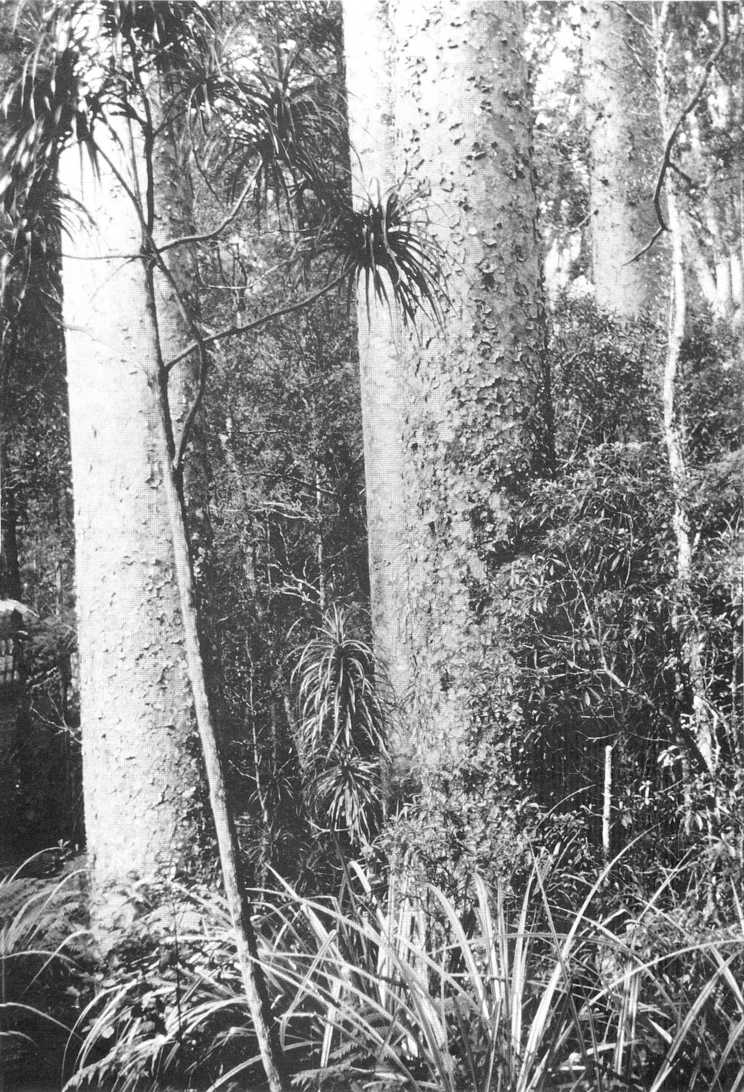
\includegraphics[width=0.66\textwidth]{graphics/figure65kauri.jpg}
	\centering
	\caption[Kauri forest interior]{Kauri (\BotanicRef{Agathis australis}[Agathis][australis]) forest interior.
	The large trunks are \IDX{kauri}s.
	The narrow-leaved shrubs are \IDX{neinei} (\BotanicRef{Dracophyllum latifolium}[Dracophyllum][latifolium]), and the narrowleaved ground herbs \IDX{kauri grass}[kauri!grass] (\BotanicRef{Astelia trinervia}[Astelia][trinervia]).
	Puketi forest near the Bay of Islands, northern North Island.
	Photo:  J. W. Dawson.}%
	\label{fig:65kauri}
\end{SCfigure}
Their crowns form a high canopy at about \SIrange{35}{40}{\metre} and plant growth below this is often rather sparse.
Most of the tree species of the non-kauri forests are present however, including \IDX{rimu}, \IDX{taraire}, \IDX{tawa}, \IDX{towai} and \IDX{northern rata}[rata!northern], but they tend to be rather small-crowned and spindly.
Most of the shrubs and ground plants are found elsewhere, although some are particularly abundant in \IDX{kauri forest}[kauri!forest]: \IDX{toru} (\BotanicRef{Toronia toru}[Toronia][toru]), \IDX{neinei} (\BotanicRef{Dracophyllum latifolium}[Dracophyllum][latifolium]) \IDX{mairehau} (\BotanicRef{Phebalium nudum}[Phebalium][nudum]) and a terrestrial form\footnote{The terrestrial form is probably a distinct species. (See~\cite{eagle1982trees}).} of the normally epiphytic \BotanicRef{Brachyglottis} (\IDX{kohurangi}, \BotanicRef{Senecio kirkii}[Senecio][kirkii]).
Particularly conspicuous where they occur are the often huge tussocks of `\IDX{kauri grass}[kauri!grass]' (\BotanicRef{Astelia trinervia}[Astelia][trinervia]) and the sedge \IDX{mapere} (\BotanicRef{Gahnia xanthocarpa}[Gahnia][xanthocarpa]).

The fallen leaves, bark flakes and twigs of the \IDX{kauri}s form a litter poor in nutrients, which is slowly decayed by fungi rather than the more nutrient-demanding bacteria.
In these circumstances the litter accumulates to considerable depths, sometimes up to \SI{3}{\metre} near large trees.
The litter becomes very acidic and this promotes heavy leaching from the upper layers of the soil and the formation of a thick concrete like iron pan at a lower level.
The impervious nature of this can result in quite swampy conditions.

\IDX{Kauri}[kauri]s not only establish on less fertile soils; they also greatly impoverish them.
It is not surprising, then, that there is little regeneration of \IDX{kauri}s on the floor of a \IDX{kauri forest}[kauri!forest].
Cockayne\footnote{\cite{cockayne1928vegetation}} thought that this was due to there being insufficient light on the forest floor, but more recent studies suggest that it results from the infertility of the litter and soil and perhaps also to competition from the roots of the mature trees.\footnote{\cite{bieleski1959factors}}
Whatever the cause, the lack of regeneration shows that \IDX{kauri}s are unable to replace themselves in closed forests, and Cockayne postulated that the climax forest would be one without \IDX{kauri}s in which the dominance would probably be assumed by \IDX{taraire}.

However, the study of soils under some \IDX{kauri forest}[kauri!forest]s has revealed a succession of `fossil soils' at depth which contain \IDX{kauri gum}[kauri!gum] and other remains.
This demonstrates a succession of \IDX{kauri forest}[kauri!forest]s on the same site.
As each generation of \IDX{kauri}s died out, perhaps as a result of conditions they themselves induced, the various flowering trees and shrubs remaining or following would restore soil fertility sufficiently to permit the establishment of a new \IDX{kauri} generation.

In some cases buried \IDX{kauri} logs are all aligned in the same direction, indicating destruction by a cyclone.
Bieleski\footnote{\cite{bieleski1959factors}} suggests that the upturned roots of the blown over \IDX{kauri}s would break through the iron pan, improve the drainage of the soil and so allow a new sequence to commence.

At present there is extensive \IDX{kauri} regeneration in areas where forests have been logged or burnt in European times.
The pioneer phase is dominated by the light-demanding \IDX{manuka} (\BotanicRef{Leptospermum scoparium}[Leptospermum][scoparium]) followed by \IDX{kanuka} (\BotanicRef{Kunzea ericoides}[Kunzea][ericoides]).
Numerous \IDX{kauri} seedlings and those of other species develop under the \IDX{kanuka} canopy and as the latter opens out the \IDX{kauri}s grow through and overtop it.

Another type of shrubland widespread in the north is found on terrain known as `gumland'.\footnote{\cite{esler1975gumland}}
The \IDX{kauri forest}[kauri!forest]s preceding the gumland vegetation left in the soil considerable quantities of resin, which was gathered intensively following European settlement for the making of polishes and varnishes.
The soil is highly infertile and it is thought that repeated fires in both Maori and European times have led to the present degraded vegetation.
\IDX{Manuka}[manuka] (\BotanicRef{Leptospermum scoparium}[Leptospermum][scoparium]) is quite common, although stunted, and other characteristic shrubs are \BotanicRef{Dracophyllum lessonianum}[Dracophyllum][lessonianum] and the strikingly yellow-flowered \IDX{kumarahou} or `Gumdigger's Soap'\footnote{Kumarahou flowers rubbed together with water form a sort of lather.} (\BotanicRef{Tomaderris kumeraho}[Tomaderris][kumeraho]).
Among herbs, sedges and the umbrella fern (\BotanicRef{Gleichenia tirtinata}[Gleichenia][tirtinata]) are prominent.
Undoubtedly the gumlands would have to be free of fire for a very long time before \IDX{kauri forest}[kauri!forest]s could return.

Finally, the most puzzling sites containing \IDX{kauri} remains are swamps, as \IDX{kauri}s do not grow in such sites except sometimes marginally.
Not only is it common to find \IDX{kauri gum}[kauri!gum] in Northland swamps, but it is often located in several distinct layers indicating a succession of forests, presumably at times when drainage was good, alternating with treeless swamps.

Cheeseman,\footnote{\cite{cheeseman1896flora}} when considering the swamps of the low lying sandy peninsula leading to North Cape, was the first to suggest an explanation involving cyclical changes in height of the land above the sea.
He was thinking in terms of raising and lowering of the land, but, although the effect was the same, we now know that it was a matter of raising and lowering of the sea level.
At each glacial period during the recent (or perhaps current) ice age, sea levels dropped by up to \SI{100}{\metre} as large amounts of water were locked up in ice.
Then, with each interglacial, ice would melt to varying extents and the sea level would rise again.
With the lowered sea level, drainage of the swamps would improve and \IDX{kauri forest}[kauri!forest] would establish; with a raised sea level the forests would disappear as drainage deteriorated sometimes to the extent of inundation by the sea.

If this explanation for the former existence of \IDX{kauri forest}[kauri!forest]s on currently swampy sites is correct it presents us with a curious contradiction: on such sites the \IDX{kauri}, now restricted to the warmest part of New Zealand, flourished during glaciations and disappeared during interglacials!

\subsection{Mangrove Forest}

\IDX{Mangrove}[mangrove] is the term applied to a number of small trees, mostly tropical, which grow between the tides in shallow seas bordering sheltered coasts.
In New Zealand we have only one species, \IDX{manawa} (\BotanicRef{Avicennia resinifera}[Avicennia][resinifera]).
The derivation of the species' name is interesting; it was applied by the botanists on Cook's first voyage, in the mistaken belief that the bits of floating \IDX{kauri gum}[kauri!gum] they observed came from nearby \IDX{mangrove}s.

Like the \IDX{kauri}, \IDX{manawa} is restricted to the warmest part of the country reaching the Bay of Plenty in the east and Kawhia in the west.
Towards its southern limits it is no more than a shrub, but further north \IDX{manawa} can be a tree up to \SI{10}{\metre} high forming low forests with a close canopy.
For the most part these forests contain no other species of flowering plants.

\subsection{Fresh Water Swamp Forest}

In the lowlands throughout New Zealand, swamp forest often occurs in localised areas depressed below the general level of the landscape.
Such depressions can be found in the irregular terrain of volcanic and formerly glaciated areas; in areas where land blocks have sunk along faults; where meandering rivers have changed their courses; and between consolidated sand dunes.


If there is some depth of water initially, then water plants begin the succession.
Some of these are completely submerged and grow on the bottom of the pond or lake; others are free floating at the surface.
Where the latter grow near the shore they gradually reduce the water depth with the accumulation of their own remains and the streamborne silt they trap.
In the shallower water which results, some aquatic plants with submerged roots but foliage raised well above the water enter the progression.
Notable among these is the \IDX{raupo} (\BotanicRef{Typha orientalis}[Typha][orientalis]).
The \IDX{raupo} in turn raises the ground level to coincide (more or less) with the water level and then gradually gives way to the so-called New Zealand flax, \IDX{harakeke} (\BotanicRef{Phormium tenax}[Phormium][tenax]) intermixed with \IDX{toetoe} (\BotanicRef{Cortaderia toetoe}[Cortaderia][toetoe]) and \IDX{purei} (\BotanicRef{Carex secta}[Carex][secta]).
This stage is an impressive sight when the \BotanicRef{Phormium} is bearing its spiky reddish flower heads and the \IDX{toetoe} its creamy yellowish plumes.
In time shrubs tolerant of poorly drained soil become established --- \IDX{manuka} (\BotanicRef{Leptospermum scoparium}[Leptospermum][scoparium]), \IDX{koromiko} (\BotanicRef{Hebe stricta}[Hebe][stricta]), \IDX{karamu} (\BotanicRef{Coprosma robusta}[Coprosma][robusta]) and a variety of divaricating shrubs including several coprosmas.
The first trees to appear are often \IDX{ti kouka} (\BotanicRef{Cordyline australis}[Cordyline][australis], \IDX{cabbage tree})\figureref{\fullref{fig:66cabbagetree}}, so characteristic of many New Zealand landscapes.
Finally come the trees of the closed forest, the most prominent of these being \IDX{kahikatea} (\BotanicRef{Dacrycarpus dacrydioides}[Dacrycarpus][dacrydioides]).
In \IDX{kahikatea} swamp forest\figureref{\fullref{fig:67kahikatea}}, as it is often called, the trunks of the dominant trees may be close-set and exceedingly tall with relatively small grayish green crowns.
\begin{figure}[t]
	% Outer minipage scaled to limit width.
	% Inner minipages scaled so the images have the same height.
	\begin{minipage}[t]{\textwidth}
		\begin{minipage}[t]{(\textwidth-\fgap) * \real{0.395}}
			\centering
			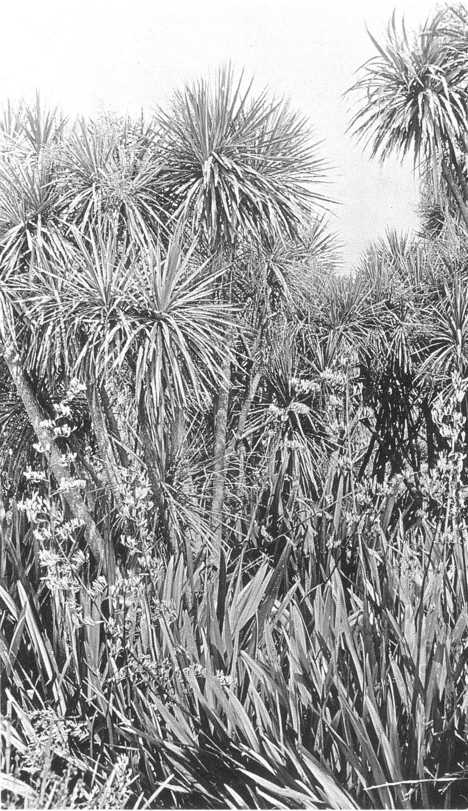
\includegraphics[width=\textwidth]{graphics/figure66cabbagetree.jpg}
			\caption[Swamp with cabbage trees]{Swamp with \IDX{ti kouka} (\BotanicRef{Cordyline australis}[Cordyline][australis], \IDX{cabbage tree}) and New Zealand `flax', \IDX{harakeke} (\BotanicRef{Phormium tenax}[Phormium][tenax]). Near Kaeo, northern North Island.
			Photo: J. W. Dawson.}%
			\label{fig:66cabbagetree}
		\end{minipage}\hspace{\fgap}%
		\begin{minipage}[t]{(\textwidth-\fgap) * \real{0.605}}
			\centering
			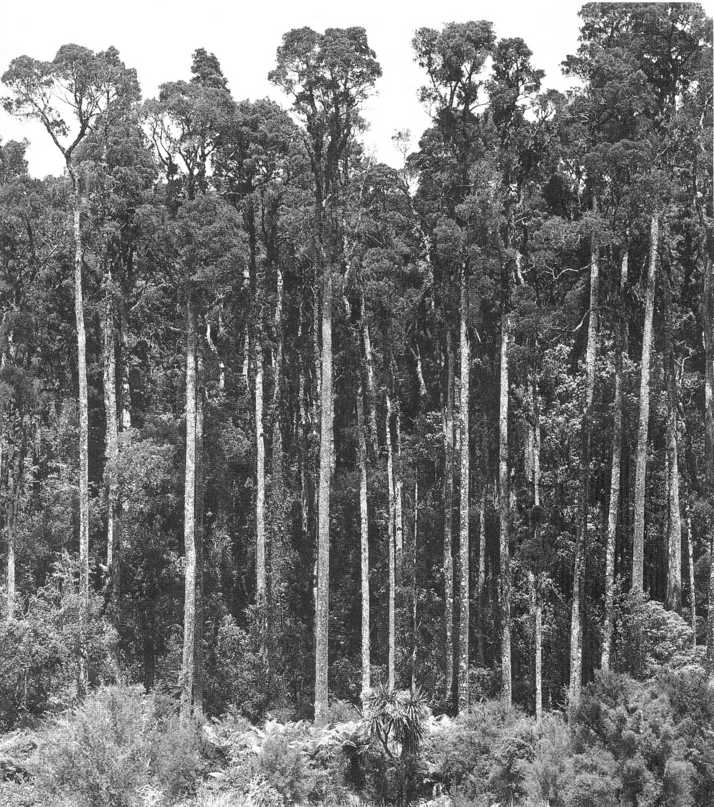
\includegraphics[width=\textwidth]{graphics/figure67kahikatea.jpg}
			\caption[Exterior view of kahikatea swamp forest]{Exterior view of \IDX{kahikatea} (\BotanicRef{Dacrycarpus dacrydioides}[Dacrycarpus][dacrydioides]) swamp forest.
			Harihari, west coast, South Island.
			Photo: J. H. Johns.}%
			\label{fig:67kahikatea}
		\end{minipage}
	\end{minipage}
\end{figure}
In the North Island, and northern parts of the South Island, \IDX{pukatea} (\BotanicRef{Laurelia novae-zelandiae}[Laurelia][novae-zelandiae]) is a common associate of \IDX{kahikatea} and in this type of forest often has well-developed plank buttresses which extend into roots raised above the forest floor with shield-like pneumatophores here and there.
The \IDX{swamp maire} (\BotanicRef{Syzygium maire}[Syzygium][maire]) has a similar distribution, but it is a smaller tree.

There is an often rather open undergrowth of small-leaved and large leaved shrubs, many of which persist from earlier stages in the succession, and sedges are prominent among the forest floor plants.
Herbaceous and woody epiphytes are often common and among the vines \IDX{kiekie} (\BotanicRef{Freycinetia baueriana var.\ banksii}[Freycinetia][baueriana var.\ banksii]) is particularly abundant, covering the forest floor in places and completely obscuring the trunks of trees up to a considerable height\figureref{\fullref{fig:32kiekie}}.

Over time, when the soil has built up sufficiently above the water table, the swamp forest will give way to ordinary conifer broadleaf forest.

\subsection{Bog Forest}

Bogs, although similar to swamps in that they are waterlogged, are much less fertile and much more acid, and the slow breakdown of plant remains which results from these conditions leads to the build up of peat, often with peat moss (\BotanicRef{Sphagnum}) playing a prominent role.
The greater fertility of swamps is due to the fact that most of their water content comes either from streams or from ponds or lakes fed by streams.
The latter contain minerals dissolved from the rocks and soils through which they pass and in times of flood they may also carry quantities of fertile silt.
Bogs on the other hand are found mostly in high rainfall areas and most of their water comes as rain, which is devoid of nutrients.
Their other characteristics follow from this.

Raised bogs have convex surfaces and consequent outward drainage.
They are best developed in the Waikato and parts of Southland and they may become established on former swamps.

In the North Island forested bogs are largely restricted to middle altitudes on the central volcanic plateau near to Mt. Ruapehu.
In the South Island they are common on the lowlands of the wet western side and also in Southland and Fiordland.

Bog forest is low in stature, up to 15 m, and the usual dominant tree is \IDX{silver pine} (\BotanicRef{Lagarostrobos colensoi}[Lagarostrobos][colensoi])\footnote{Silver pine is replaced by \IDX{yellow silver pine} (\BotanicRef{Lepidothamnus intermedius}[Lepidothamnus][intermedius]) in western Southland and Fiordland.} intermixed with small trees of the mountain celery pine (\BotanicRef{Phyllocladus aspleniifolius var.\ alpinus}[Phyllocladus][aspleniifolius var.\ alpinus]).
\IDX{Rōhutu}[rōhutu] (\BotanicRef{Neomyrtus pedunculata}[Neomyrtus][pedunculata]) may be prominent in the subcanopy and large tussocks of \IDX{kakaha} (\BotanicRef{Astelia fragrans}[Astelia][fragrans], \IDX{bush flax}) may be abundant on the forest floor.
The progression from bog to bog forest has been studied in South Westland where islandlike patches of bog, known locally as \IDX{pakihi}, are scattered in forest on the lowland gravel plain.
The \IDX{pakihi} vegetation is dominated by the rush-like \BotanicRef{Empodisma minus}[Empodisma][minus] with the sedge \BotanicRef{Baumea teretifolia}[Baumea][teretifolia], the umbrella fern, \BotanicRef{Gleichenia circinata}[Gleichenia][circinata] and various other small herbs.
Stunted shrubs of \IDX{manuka} and \IDX{inanga} (\BotanicRef{Dracophyllum longifolium}[Dracophyllum][longifolium]) are scattered throughout.
In the gradation from bog to forest there is firstly a zone of \IDX{manuka} of small tree size under which silver pine in particular establishes.
In the next zone, silver pine has formed a canopy above the \IDX{manuka}.
Silver pine is itself overtopped by \IDX{rimu} (\BotanicRef{Dacrydium cupressinum}[Dacrydium][cupressinum]) in the next zone\figureref{\fullref{fig:68transition}}.

\begin{SCfigure}[1.0][t]
	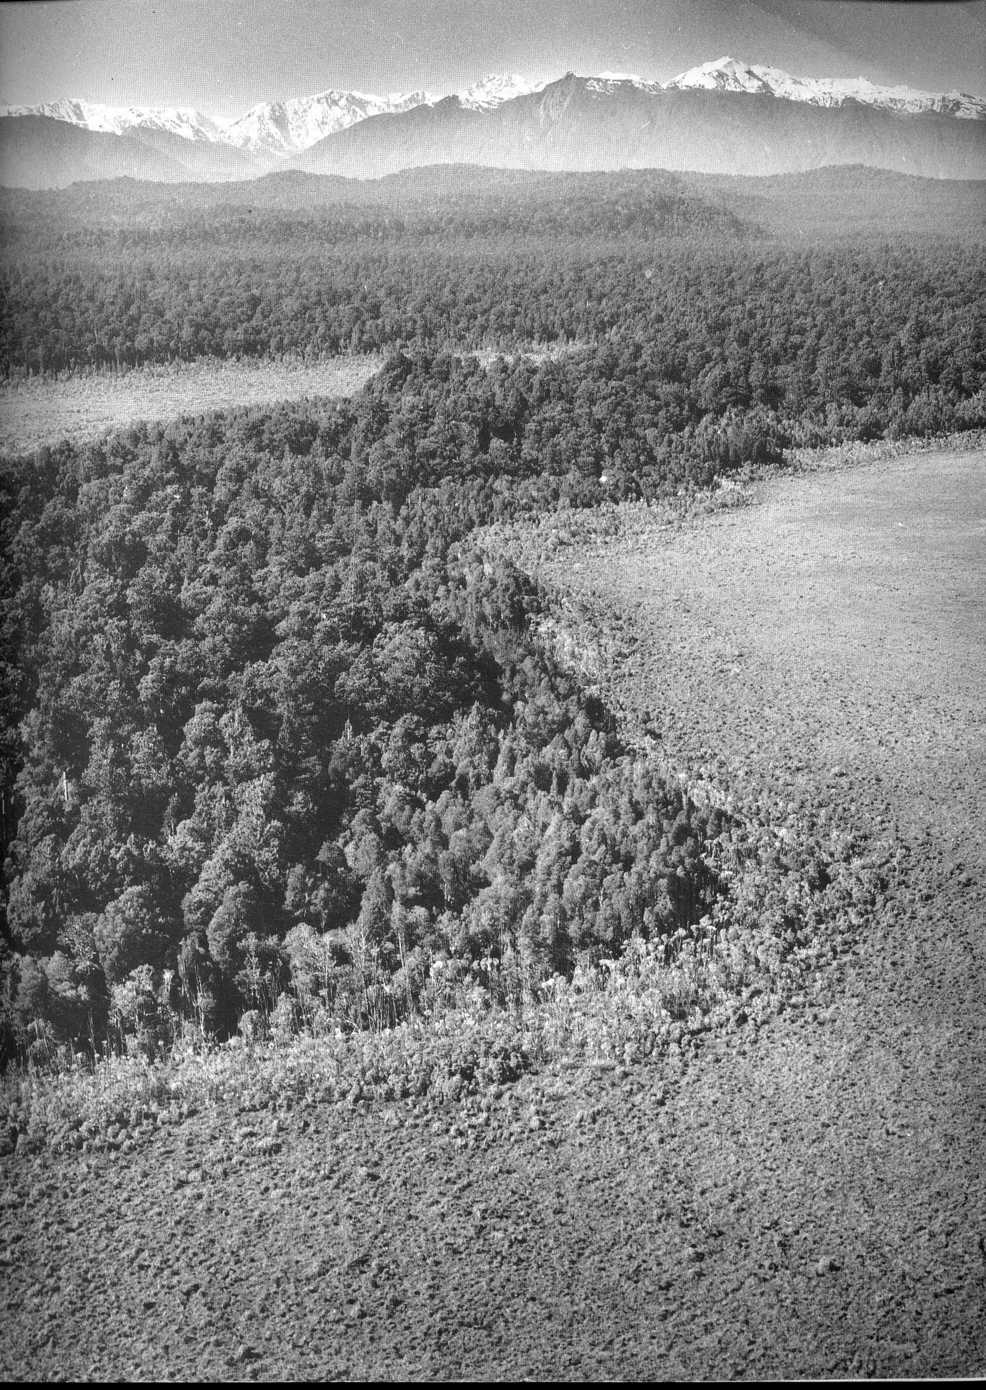
\includegraphics[width=0.66\textwidth]{graphics/figure68transition.jpg}
	\centering
	\caption[Aerial view of the transition from pakihi bog through silver pine to rimu]{Aerial view of the transition from \IDX{pakihi} bog through \IDX{silver pine} (\BotanicRef{Lagarostrobos colensoi}[Lagarostrobos][colensoi]) dominated forest to \IDX{rimu} (\BotanicRef{Dacrydium cupressinum}[Dacrydium][cupressinum]) dominated forest on better drained terrain.
South Westland.
	Photo: J. H. Johns.}%
	\label{fig:68transition}
\end{SCfigure}

As with \IDX{kahikatea} swamp forest, it seems probable that as the soil level builds up and soil moisture declines sufficiently, the progression ultimately leads to the general conifer broadleaf forest of the region.
Any trend towards increased regional rainfall would, of course, slow or even reverse such a progression.

Mark and Smith\footnote{\cite{mark1975lowland}} concluded that the \IDX{pakihi} in their south Westland study area had never previously supported forest, but Rigg,\footnote{\cite{rigg1962pakihi}} who studied \IDX{pakihi}s in north Westland, suggested, on the evidence of buried logs, that forests (probably dominated by \IDX{rimu}) did formerly occupy such terrain and that there was possibly a succession of such forests.
The soil of these \IDX{pakihi}s is highly leached and infertile with a well developed iron pan, which also suggests a previous forest which provided an acid litter.
Rigg proposes, as one possibility, that the podocarp forests would have died out as a result of the reduced soil fertility and, presumably, the impeded drainage they themselves induced.
Between successive forests a regeneration sequence similar to that described for South Westland would have taken place.
This hypothesised forest-bog-forest cycle is similar to the forest/swamp/forest cycle proposed for some \IDX{kauri} localities.

As with the gumlands of Northland, many of the \IDX{pakihi}s of Westland have been repeatedly burnt in both Maori and European times.
